\documentclass[Main]{subfiles}

\begin{document}


\section{Anvendte metoder}

Projektet er udviklet på metoden om Unified Process\cite[s. 74]{Larman}, også vist på Figur \ref{Fig:UP}.

\begin{figure}[H]
\centering
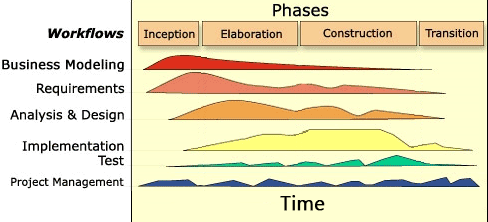
\includegraphics[scale=0.6]{Iterations}
\caption{Unified Process}
\label{Fig:UP}
\end{figure}



\subsection{Faser}
I starten skulle der ligges en del arbejde i, at finde den rigtige drone der både havde open source kode og ikke var alt for dyr (Business Modeling).
Da først dronen var valgt, kunne Kravspecifikationen\cite{Kravspec} skrives ud fra overvejelser om, hvordan projektet kunne blive en realitet (Requirements).
Da kravene var på plads blev der åbnet op for både koden til dronen og senderen/modtageren og en struktur herpå kunne formes (Analysis \& Design).

Efter forståelse for systemet blev implementeringen af Kravspecifikaitonen begyndt og testet, så de enkelte elementer virkede efter hensigten (Implementation og Test).
Til sidste var der et funktionelt produkt (Deployment)\fxnote{Vag formulering}.




\subsection{Use Cases}
For at beskrive hvad projektet skal kunne, er der anvendt Use Cases.
Disse er meget anvendelige til udvikling af produkter, da disse specificerer hvordan systemet skal opføre sig i forskellige situation.
På denne måde synliggøres systemets krav og funktionalitet.
Beskrivelse af Use Cases følger en strikt skabelon, der skrives i punktform og i et let forståeligt sprog.














\end{document}